
\documentclass[preprint,12pt]{article}


\makeatletter


\usepackage[utf8]{inputenc} % allow utf-8 input
\usepackage[T1]{fontenc}    % use 8-bit T1 fonts
\usepackage[hidelinks]{hyperref}       % hyperlinks
\usepackage{url}            % simple URL typesetting
\usepackage{booktabs}       % professional-quality tables
\usepackage{amsfonts}       % blackboard math symbols
\usepackage{nicefrac}       % compact symbols for 1/2, etc.
\usepackage{microtype}      % microtypography
\usepackage{xspace}
\usepackage{enumerate}
\usepackage{xcolor}
\usepackage{graphicx}

\newcommand{\nb}[1]{\textcolor{red}{#1}}
\urlstyle{rm}

\newcommand{\labeltrue}{\textsc{like}\xspace}
\newcommand{\labelfalse}{\textsc{dislike}\xspace}

\title{Measuring performance of a classification method in a way that can be easily explained in words}

% The \author macro works with any number of authors. There are two commands
% used to separate the names and addresses of multiple authors: \And and \AND.
%
% Using \And between authors leaves it to LaTeX to determine where to break the
% lines. Using \AND forces a line break at that point. So, if LaTeX puts 3 of 4
% authors names on the first line, and the last on the second line, try using
% \AND instead of \And before the third author name.

\author{David J. T. Sumpter \\ Department of Information Technology, Uppsala University, Sweden}

\begin{document}


% \nipsfinalcopy is no longer used

\maketitle

\begin{abstract}
A good performance metric can be stated in words. The area under the ROC curve (AUC) is the probability that a randomly chosen image of a cat scores higher than a randomly chosen image without one. But this is rarely the question we face in practice, and adding images that are easy to reject pushes it towards one. We propose a metric that answers the question we usually want answered: when the algorithm is tuned so that it can no longer distinguish the images it labels as cats from the images that really contain cats, how often does an image labelled as a cat actually contain one? To construct it, the decision threshold is first set so that a randomly chosen labelled image and a randomly chosen real cat are equally likely to have the higher score. The metric is then the precision at this threshold, which we call {\it precision at the indistinguishability threshold}. Unlike AUC, it is unaffected by adding easy cases and, unlike the F1-score, its value can be explained directly in words. We derive exact relationships with precision, recall and F1, showing that at this threshold more images are always labelled as cats than there are cats, so that recall exceeds precision, and that the threshold generally differs from the one that maximises F1. On a benchmark data set of mammograms, two classifiers with the same AUC differ by 13 percentage points in precision at the indistinguishability threshold.
\end{abstract}

\section*{Introduction}

Imagine you have created an algorithm (a machine learning model) that assigns a score, predicting whether an entity belongs to one of two classes (positive and negative). For example, the input might be a picture and the output whether or not the picture contains a cat. The scores are larger if your algorithm evaluates the object as more likely to belong to the positive class (i.e if it labels the image as more likely to contain a cat). Such a scoring system explicitly underlies, for example, logistic regression, the output of a neural network and discriminant analysis \cite{smlbook}. Other, non-parametric machine learning methods, such as $k$-nearest neighbours \cite{fix1989discriminatory}, don't have an explicit score, but often have a parameter (e.g. $k$) which can be tuned in a way that mimics a threshold. 

\begin{figure}[p]
\centering
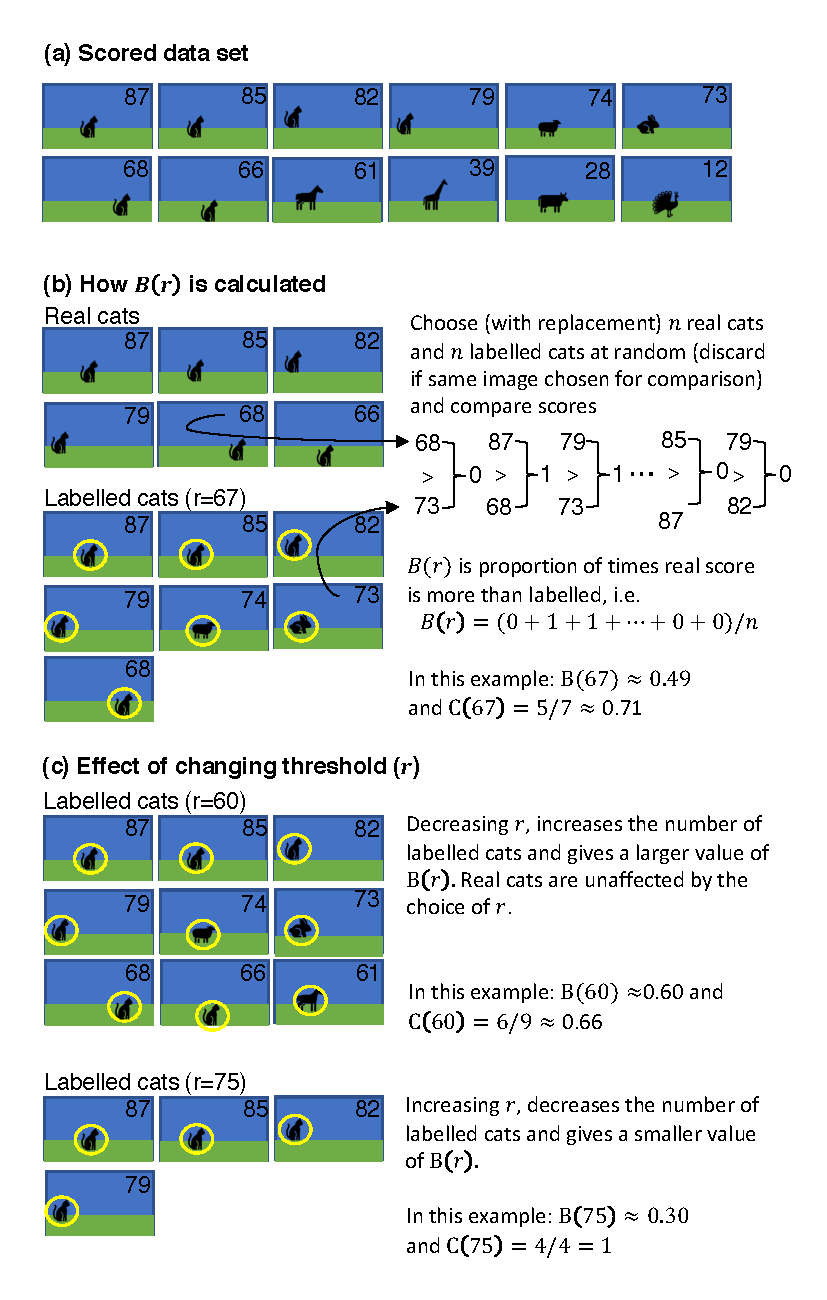
\includegraphics[scale=1]{Figures/FindCats.pdf}
\caption{Illustration of the method described in this paper} \label{fig:methodill}
\end{figure}

The method we suggest for evaluating performance in this article is as follows. We start, in figure \ref{fig:methodill}a, with a data set in which every image is assigned a score. We first investigate what happens when we set a threshold score, $r$, above which we label the image as containing a cat (positive), below which we label the image as not containing a cat (negative). For any given threshold we compare those images which we label as cats (given the threshold) with those containing real cats. Specifically, we choose (with replacement) $n$ real cats and $n$ labelled cats at random and compare scores (figure \ref{fig:methodill}b). In cases where we happen to pick the same two images, we pick two new images for that particular comparison. This gives a measure $B(r)$: the probability a real cat scores more than a labelled cat for threshold $r$.

We then identify a specific threshold score, $r_b$, such that if we were to choose one image that the algorithm classifies as containing a cat and a second image that really does contain a cat, then the probability that the score of the image containing the cat is the largest of the two scores is 50\%. We define this as $r_b$, where  $B(r_b) \approx 0.5$. In the example, in figure \ref{fig:methodill}b $r_b=67$. A smaller threshold gives $B(r) > 0.5$ and a larger threshold gives $B(r) < 0.5$ (figure \ref{fig:methodill}c). We call $r_b$ the {\it indistinguishability threshold}: because the set comprised of false positives (FP) and true positives (TP) is indistinguishable from the set of TPs and false negatives (FN). When $r=r_b$, if we pick (at random) two images from our data set, one which is labelled as a cat and the other that is known to contain a cat, then the probability that the algorithm will assign the image with the cat the highest score is one half.

To measure the performance of your algorithm, simply calculate the proportion of images the algorithm classifies as containing a cat do actually contain a cat. We denote this measure $C(r_b)$ and call it {\it precision at the indistinguishability threshold}.

There already exist a number of ways of evaluating classification algorithms. Wikipedia lists a somewhat bewildering array of 17 tests, with a total of 27 different names, for such problems.  The most commonly used method is the area under the Receiver-Operator Curve, commonly referred to as AUC \cite{obuchowski2018receiver, vanderlooy2008critical, majnik2013roc}. Much of its appeal lies in its simple interpretation: it is the probability that a randomly chosen member of the positive class scores higher than a randomly chosen member of the negative class \cite{bamber1975area, hanley1982meaning}. But AUC also has well-known limitations. It summarises performance over all thresholds, including those at which a classifier would never be used \cite{lobo2008auc}; it can favour one classifier over another even when the other performs better over almost all thresholds \cite{hand2009measuring}; and when the negative class is large it can give an overly optimistic view of how well a classifier identifies the positive class \cite{davis2006relationship, saito2015precision}. Responses to these limitations include the partial AUC, which restricts attention to a range of false positive rates \cite{mcclish1989analyzing, dodd2003partial, carrington2020new}, and precision-recall curves, which focus on how often positive labels are correct \cite{davis2006relationship, saito2015precision, flach2015precision}.

Another popular choice is the F1-score \cite{sasaki2007truth}, which seeks to avoid a problem inherent in AUC when applied to unbalanced data \cite{smlbook}. Unlike AUC, the F1-score has no simple interpretation in words. Hand and Christen showed that it is a weighted arithmetic mean of precision and recall in which the weights depend on the classifier being evaluated, rather than on the problem \cite{hand2018note}, and Hand, Christen and Kirielle proposed a transformation of it, F*, with a more direct interpretation \cite{hand2021f}.

Measures such as precision and the F1-score are calculated at a particular threshold, so their values depend on how that threshold is chosen. Common choices include the threshold which maximises the F1-score \cite{lipton2014optimal, koyejo2014consistent}; the threshold at which precision equals recall, known as the break-even point or R-precision \cite{manning2008introduction}; the threshold which maximises Youden's index, the difference between the true and false positive rates \cite{youden1950index}; and, when the costs of the two types of error are known, the threshold which minimises the expected cost \cite{elkan2001foundations}. In the quantification literature, which aims to estimate the number of members of each class, thresholds are also chosen by simple rules, such as setting the true positive rate to one half \cite{forman2008quantifying}. Hern\'andez-Orallo, Flach and Ferri showed that many performance measures can be understood as the combination of a method for choosing a threshold and a measure of loss at that threshold \cite{hernandez2012unified}. In this paper, we propose a new method for choosing a threshold, the indistinguishability threshold, and argue that precision at this threshold, $C(r_b)$, provides an easy to understand alternative to the F1-score, which avoids many of the problems inherent to AUC.

\section*{Results} 


\subsection*{Area under the curve} 
\label{sec:AUC}

We now show that the area under the ROC curve (AUC) measures the probability that a member of the positive class scores higher than a member of the negative class. This has been known since Bamber \cite{bamber1975area}, and was made widely known by Hanley and McNeil \cite{hanley1982meaning}. We retell it here since the argument, which compares the scores of randomly chosen pairs of members, is the same one we use to construct a new measure in the sections that follow.

To calculate this probability, we pick one member of the positive class at random and one member of the negative class at random and look to see which of them has the higher score. As a concrete example, imagine an algorithm is shown two images, one which contains a cat, another which does not. The task is to pick the image containing the cat. We call this probability 
\[
A = P(S_P>S_N)
\]
where $S_P$ is the score of a randomly chosen positive member and $S_N$ is the score of a randomly chosen negative member. The value of $A$ can be measured directly, simply by randomly picking pairs of members of negative and positive classes and testing which scores higher. The test outcome is then the proportion of cases in which the positive member receives a higher value than the negative member.

We can also measure the paired comparison test over all our scores. Let $F_P(r)$ be the cumulative distribution of scores of the positive class, i.e. 
\begin{equation}
F_P(r) = P(S_P < r) = \int_{s=-\infty}^{r} f_P(s) ds \label{eq:ScorefPr}
\end{equation}
where $f_P(r)$ is thus the probability density function of $S_P$. Likewise, we let $F_N(r)$ to be the cumulative distribution of scores the negative class, i.e. 
\begin{equation}
F_N(r) = P(S_N < r) = \int_{s=-\infty}^{r} f_N(s) ds \label{eq:ScorenPr}
\end{equation}
The value $A=P(S_P>S_N)$ can be written as the double integral
\begin{equation}
A = \int_{r=-\infty}^{\infty} \int_{s=r}^{\infty}  f_N(r) \cdot  f_P(s) ds dr  \label{eq:SPgreaterSN}
\end{equation}
which is equivalent to
\begin{equation}
A = \int_{r=-\infty}^{\infty}  f_N(r)  \int_{s=r}^{\infty}  f_P(s) ds dr  = \int_{r=-\infty}^{\infty}  f_N(r) \cdot  \left(1 -  F_P(r) \right) dr \label{eq:SPgreaterSN2}
\end{equation}
We can use this equation to calculate $A$ by numerical integration. 

We can also use this formulation to derive the equivalence between the $A$ test and AUC. To do so, note that the true positive rate for a given threshold $r$ is given by $v(r)=1-F_P(r)$ and that the false positive rate for a given threshold $r$, is given by $u(r)=1-F_N(r)$. Then we see that
\[
A  =  \int_{r=-\infty}^{\infty} v(r) f_N(r) dr  
\]
which by change of variable gives
\begin{equation}
A  = \int_{u=0}^{1} v \left( u^{-1}(u) \right) du  \label{eq:AUCdef}
\end{equation}
where $u^{-1}$ denotes the inverse of the function $u(r)$, so that $v(u^{-1}(u))$ is the true positive rate at the threshold where the false positive rate is $u$. Thus $A$ is also the area under the ROC curve (which is defined by the right hand side of equation \ref{eq:AUCdef}).

\begin{figure}[tp]
\centering
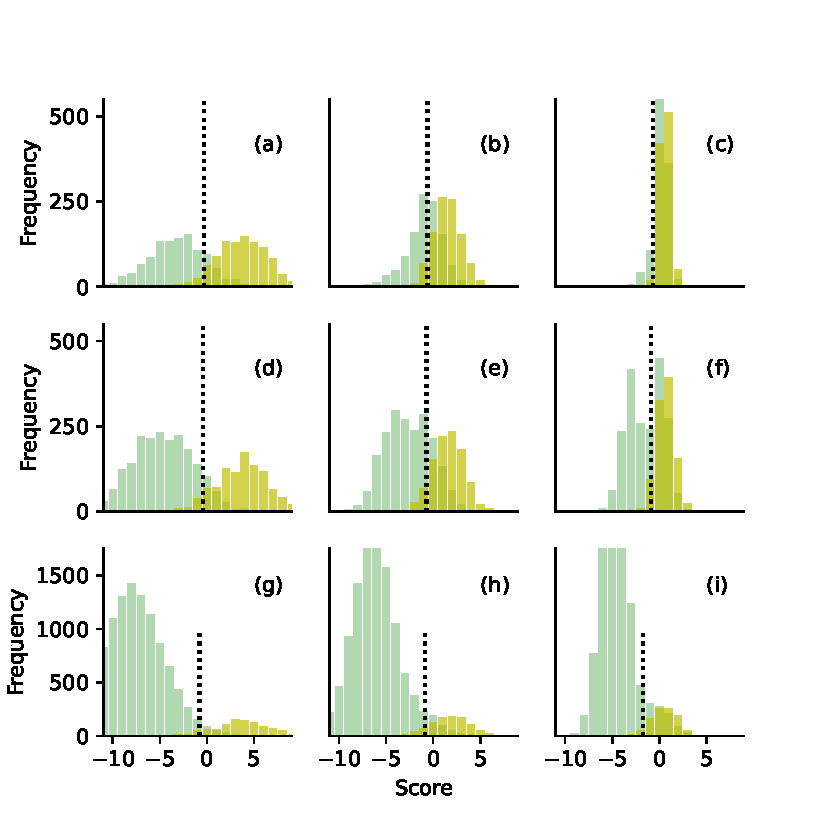
\includegraphics[scale=1]{Figures/Distribution.pdf}
\caption{The score distributions for the nine example data sets we look at here. Green are members of the negative class, yellow members of the positive class. The dotted line shows $r_b$, the solution $B(r)=1/2$ (see equation \ref{balanced})} \label{fig:Distribution}
\end{figure}

\subsection*{Artificial data sets}

To see how $A$, and the further measures introduced below, behave in practice, we use nine artificial data sets, shown in figure \ref{fig:Distribution}. The positive class ($Y_i=1$) is created by first generating 1000 input values, $X_i$, with a mean $m_p=10$ and standard deviation $\sigma_p=2$. Similarly, the negative class ($Y_i=-1$) consists of 1000 `difficult' data points with values, $X_i$, which have mean scores (a,d,g) $m_n=5$; (b,e,h) $m_n=7$; (c,f,i) $m_n=9$ and (in all cases) standard deviation $\sigma_n=2$, along with (a,b,c) 100; (d,e,f) 1000; (g,h,i) 10000 `easy' data points, $X_i$, with mean 2 and standard deviation 2.  We then performed logistic regression on $X_i$ to predict $Y_i$ and calculated the log-likelihood for every individual point. These log-likelihoods are taken to be the scores, $S_i$, output by the model and are plotted in figure \ref{fig:Distribution}. 

The choice of these data sets is to give a range of difficulty levels. The data in the left column correspond to relatively easy classification tasks. The overlap between the green (negative) and yellow (positive) is small. The data in the right column is much more difficult, with a large overlap in scores for negative and positive. The datasets at the bottom include a large number of `easy' to classify negative values, but the size of the overlap is only slightly increased over the datasets at the top. The data generation method and the code are available at: \href{https://github.com/soccermatics/ABC.git}{https://github.com/soccermatics/ABC.git}.

\begin{figure}[tp]
\centering
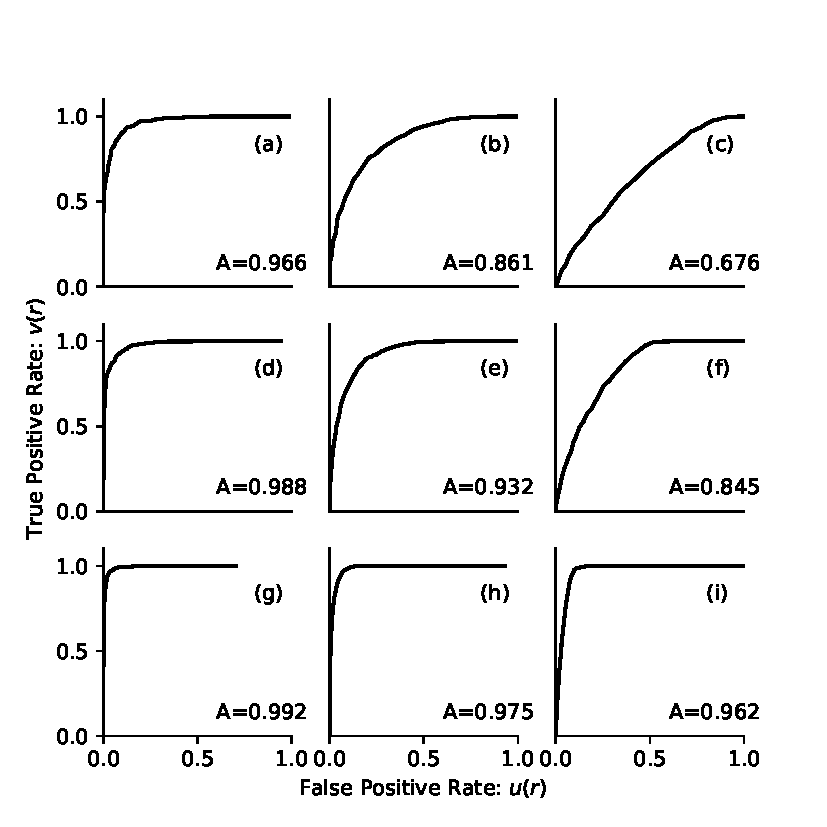
\includegraphics[scale=1]{Figures/AUC.pdf}
\caption{The area under the curve for each of the scores in figure \ref{fig:Distribution}} \label{fig:AUC}
\end{figure}

The ROC curves are shown in figure \ref{fig:AUC} for our nine data sets. The area under these curves (i.e. $A$) is shown as text within the figure. The value of $A$ is close to one when either the scores for the negative and positive class are typically different (e.g. for the score distributions shown in figure \ref{fig:Distribution} a, d and g) or there are a large proportion of 'easy' to score negative members (e.g. for the score distributions shown in figure \ref{fig:Distribution} h and i). 

These examples illustrate the limitation of $A$ as a measure. In the cases a, d and g -- where the score accurately distinguishes class members -- $A$ reflects the fact it is more likely that the algorithm picks out the positive cases correctly. But in the cases where there is an overlap between the positive and 'difficult' negative class (e.g. cases c, h and i) we see that as we add more 'easy' cases (i.e. go from c through f to i) the accuracy of the model appears to increase, despite the fact that the difficult cases are equally difficult in all three data sets. We could see this as giving a possibility for `cheating': by adding more easier cases to our data set we can appear to be improving accuracy, as measured by $A$, while no such improvement is actually occurring. 

This is why we need to be very clear about what the AUC test tells us: it tells us that if we pick one member of the positive class at random it has probability $A$ of having a higher score than one member of the negative class chosen at random. When there are a lot more 'easy'  to classify members of the negative class then a high value of $A$ is not surprising: most of the time we will randomly pick one of those members. Thus in figure \ref{fig:AUC}i  an $A$ close to one tells us very little about how well our algorithm can distinguish more difficult cases. 

\subsection*{Indistinguishability threshold}

We now change how we measure performance, by looking at how often a member of the positive class scored higher than a member that has been labelled positive. To do this, in the cat labelling problem, we first pick randomly from all images containing cats and denote the score of this image as $S_P$. Then, for a given threshold $r$, we choose randomly from all the images with that score or above, irrespective of whether or not they contain a cat. We denote this score of this image as $S_R$. We then calculate the probability 
\[
B(r) = P(S_P>S_R | S_R>r) 
\]
or, in words, the probability that a random member of the positive class scores higher than a random member of the class we have labelled as positive (i.e. has a score greater than $r$). 

Unlike the paired comparison of negatives and positives we made for $A$, it is not immediately clear how this test will help us construct a performance metric. To gain some more intuition, let's think about what happens as we change the threshold $r$. When $r$ is very large then the positively labelled set will contain more positives than negatives, but very few members of either class. As a result $P(S_P>S_R | S_R>r)$ will go towards $0$. When $r$ is small (or negative), most images are labelled positive. Nearly all members of the positive class will be included in the positively labelled set, but so too will most members of the negative class. Neither of these two situations is desirable. In the latter, we will have a lot of false positive errors and very low precision: a high proportion of those labelled positive will actually be negative. In the former case, we will have a large proportion of false negatives but very high precision: most of those which are labelled positive are actually positive.

We suggest choosing $r_b$ such that
 \begin{equation}
B(r_b) = P(S_P>S_R | S_R>r_b) = 1/2 \label{balanced}
\end{equation}
because this particular value of $r_b$ has a rather desirable property. It means that, as far as the classifier is concerned the images in the positive class are indistinguishable from those which we have labelled positive. If we pick a random member of the images we have classified as positive and a random member of the positives, these two images are equally likely to have the higher score. We can thus think of $r_b$ as being the threshold value at which the model cannot distinguish between true positives and labelled positives. The algorithm cannot distinguish reality from its own labelling. We thus refer to $r_b$ as the {\it indistinguishability threshold}. More precisely, the two sets are indistinguishable in the sense of {\it stochastic equality} \cite{vargha2000critique}: a randomly chosen member of either set is equally likely to have the higher score. Stochastic equality does not imply that the two sets have identical distributions of scores. For example, the members labelled positive could have a larger spread of scores than the members of the positive class, while still being equally likely to score higher.

To understand why this is desirable, think about a situation where we have two separate test sets of images, $Y_1$ and $Y_2$, and we want to check whether or not they have a similar distribution of scores. A solution to this problem might be to pick members from both $Y_1$ and $Y_2$ at random and compare their scores. If roughly half of the time members of $Y_1$ scored higher than members of $Y_2$ we might say that the two groups are indistinguishable. This is the idea behind the Mann--Whitney test \cite{mann1947test}: when two groups have the same distribution of scores, a randomly chosen member of one scores higher than a randomly chosen member of the other with probability one half.  In the same way,  by setting $r_b$ using equation \ref{balanced}, we are finding a threshold so that the positive class is indistinguishable from the set that is labelled positive. The vertical dotted lines in figure \ref{fig:Distribution} show the value of $r_b$ for our nine example score distribution sets. For all nine distributions the lines give a reasonable separation between the scores, lying roughly halfway between the `difficult' negative cases and the positive cases. 

The indistinguishability threshold can also be understood in terms of placement values \cite{hanley1997sampling, pepe2004analysis}. The placement value of a member, relative to the positive class, is the proportion of the positive class that scores higher than it, i.e. $v(s)$ for a member with score $s$. For the members of the positive class themselves, placement values are uniformly distributed between zero and one, and so have mean $1/2$. Since the probability that a randomly chosen positive member scores higher than a member with score $S_R$ is $v(S_R)$, $B(r)$ is the mean placement value of the members labelled positive. Setting $B(r_b)=1/2$ thus chooses the threshold at which the members labelled positive are placed, on average, exactly where the members of the positive class are placed.

A misguided (but still sometimes proposed) alternative to choosing $r=r_b$ is to instead choose $r$ such that
 \begin{equation}
\eta(r) = 1 - \eta(r) \label{standard}
\end{equation}
or, equivalently,
\begin{equation}
\eta(r) = 1/2 \label{standard2}
\end{equation}
where $\eta(r)$ is the probability that a member with score $r$ belongs to the positive class, according to an underlying model which converts scores in to probabilities. For example, when the scores are the log-odds estimated by logistic regression, the model is the logistic function
\[
\eta(r) = \frac{1}{1+\exp(-r)} = 1/2
\]
which gives $r=0$ as the threshold. Looking again at the distribution of scores in figure \ref{fig:Distribution}  we see that the size of the negative class shifts the distribution of the scores generated by the logistic regression to the left. This is undesirable, because it means that the algorithm will make more errors when easy to categorise cases are added to the data set.

The limitations of using equation \ref{standard2} to set a threshold are known, but often they are referred to as being ``caused by an unbalanced data set''. The implication is that too many members in the negative class have somehow misled us in to choosing a poor value of $r$. In our experience, students and even experienced practitioners, when confronted with this problem, either start to prune their data, removing `easy' members of the negative class, or oversample from the positive class in order to compensate. They might also draw an ROC curve and a Precision-Recall curve (see below) and try to justify, in an ad-hoc fashion, choosing a different value of the threshold $r$ on the basis of what they see in these curves.

We would argue that it is not the data set that is imbalanced, but this way of looking at it that is wrong! Specifically, it is the arbitrary choice of $r=0$ that is imbalanced, because it lies a long way from the indistinguishability threshold.


\begin{figure}[tp]
\centering
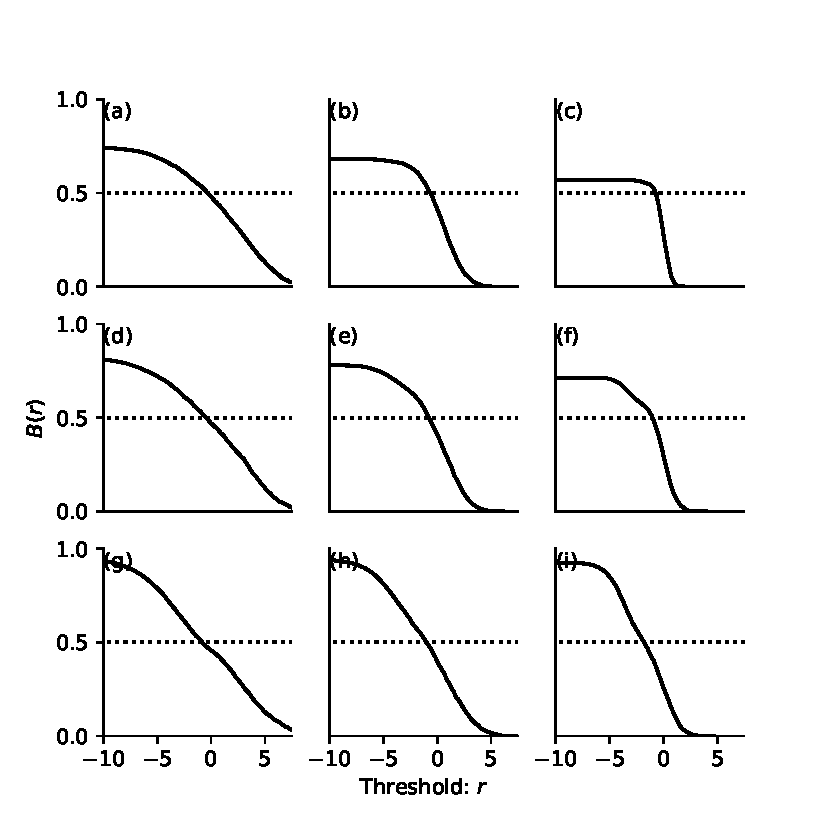
\includegraphics[scale=1]{Figures/Bplot.pdf}
\caption{Plot of $B(r)$ for our 9 example data sets. The dotted line is at $1/2$ indicates the value at which the model is balanced.}
\label{fig:Bplot}
\end{figure}



\subsection*{Precision at the indistinguishability threshold}

\label{PIT}

How often is our positive labelling correct when reality and labelling are indistinguishable? To answer this question, we define $C(r)$ to be the precision: the probability that an individual with a score greater than $r$ is in the positive class, i.e. $P(R = + | S_R > r)$ , or the probability that a positive labelling is made correctly.  Using Bayes law, we can rewrite precision in terms of false positive rate and true positive rate. Specifically,
\begin{eqnarray*}
C(r)  & = & P(R = + | S_R > r) \\
& =  &\frac{P(S_R > r | R = + ) P(R = + )}{P(S_R > r | R = + ) P(R = + ) + P(S_R > r | R = - ) P(R = - )}
\end{eqnarray*}
In this case, $P(R = + ) = P/(P+N)$ is the proportion of individuals in the positive class and $P(R = - ) = N/(P+N)$ is proportion in the negative class. Substituting $v(r)=P(S_R > r | R = + )$ (true positive rate) and $u(r) = P(S_R > r | R = - )$  (false positive rate) gives
\begin{equation}
C(r) = \frac{P v(r)}{P v(r) + N u(r)} \label{precisionP}
\end{equation}
When $N$ is much larger than $P$ then $v(r)$ has to be significantly larger than $u(r)$ for precision to have a large value. It is the ratio of true positives to all members labelled positive, with the true and false positive rates, $v(r)$ and $u(r)$, weighted by the number of members in, respectively, the positive and negative classes. 

We propose measuring precision specifically with a value of $r=r_b$, i.e. for a threshold whereby data classified as positive cannot be distinguished from data which truly is positive, i.e. we calculate $C(r_b)$. Evaluating this for the data in figure \ref{fig:Distribution} (a), (d) and (g) we get $C(r_b) \approx  0.87$. This could be considered a reasonably good performance: 87\% of the pictures the algorithm says are cats are in fact cats. For figure \ref{fig:Distribution}  (b), (e) and (h) we get $C(r_b) \approx 0.70$. This is not a great performance, but could be useable in certain applications: 70\% of the pictures the algorithm says are cats are in fact cats. Finally, for the data in figure \ref{fig:Distribution} (c), (f) and (i) we get $C(r_b) \approx  0.53$. This is poor performance, and is probably not very useful in most applications: only 53\% of the pictures the algorithm says are cats are in fact cats.

We can now see why $C(r_b)$ is preferable measure of performance over $A$. When we calculated $A$, the value was highly dependent on the number of `easy' cases. This is not the case with $C(r_b)$. By evaluating precision when the algorithm cannot distinguish reality from its own labelling, we obtain a measure of performance that doesn't depend on the number of `easy' cases. The choice of $r_b$ is theoretically motivated (in the previous section) and gives reasonable results. Before looking at how $C(r_b)$ relates to other measures of performance, we test it on real data. 


\subsection*{Two benchmark data sets}

\label{sec:benchmarks}

On a standard benchmark data set of mammograms, two classifiers with the same area under the curve (difference in $A$ of $-0.003$, 95\% interval $-0.044$ to $0.038$) differ by 13 percentage points in precision at the indistinguishability threshold (95\% interval 6 to 21 percentage points), illustrating why $C(r_b)$, rather than $A$, should be used to compare their performance.

To see how the measure behaves on real data, we applied it to two standard benchmark data sets, both obtained from OpenML \cite{vanschoren2013openml}. The Adult data set \cite{becker1996adult} contains 48,842 individuals from the 1994 US census, of whom 24\% have an annual income above \$50,000 (the positive class). The Mammography data set \cite{woods1993comparative} contains 11,183 regions of digitised mammograms, of which 260 (2.3\%) contain microcalcifications. For each data set, we trained a logistic regression and a gradient boosting classifier on a randomly chosen half of the data (stratified by class) and calculated all measures exactly from the scores on the other half. Confidence intervals were obtained by resampling the test set 1000 times, with both classifiers evaluated on the same resampled test sets. The code is available in the same repository as the code for the artificial data sets. The results are shown in table \ref{tab:benchmarks}.

\begin{table}[tp]
\centering
\footnotesize
\setlength{\tabcolsep}{3.5pt}
\begin{tabular}{lrrcccccc}
\toprule
Model & $P$ & Labelled & $C(r_b)$ & $v(r_b)$ & PRBEP & $F_1(r_b)$ & max $F_1$ & $A$ \\
\midrule
\multicolumn{9}{l}{\it Adult} \\
LR & 5844 & 8305 & 0.58 (0.57--0.59) & 0.83 & 0.68 & 0.69 & 0.69 & 0.91 \\
GB & 5844 & 7532 & 0.64 (0.63--0.65) & 0.83 & 0.72 & 0.72 & 0.73 & 0.93 \\
\multicolumn{9}{l}{\it Mammography} \\
LR & 130 & 260 & 0.35 (0.25--0.45) & 0.71 & 0.56 & 0.47 & 0.60 & 0.92 \\
GB & 130 & 194 & 0.49 (0.36--0.59) & 0.72 & 0.65 & 0.58 & 0.69 & 0.92 \\
\bottomrule
\end{tabular}
\caption{Performance on the test half of two benchmark data sets, for logistic regression (LR) and gradient boosting (GB). $P$ is the number of positives in the test set and `Labelled' the number labelled positive at the indistinguishability threshold $r_b$. $C(r_b)$ is given with a 95\% bootstrap interval. PRBEP is the precision (equal to the recall) at the precision-recall break-even point.}
\label{tab:benchmarks}
\end{table}

The measure can be reported in the same plain language as in the rest of this article. For gradient boosting on the Mammography data, for example: {\it when the algorithm is tuned so that the regions it flags cannot be distinguished from the regions that really contain microcalcifications, 49\% of the flagged regions contain microcalcifications} (95\% confidence interval 36--59\%), and 72\% of the regions containing microcalcifications are flagged.

The data also illustrate the limitation of $A$ discussed in the section {\it Area under the curve}. Removing the half of the test negatives with the lowest scores, i.e. the easiest cases, reduced $A$ by between 0.04 and 0.09 but left $C(r_b)$ unchanged, since none of these members are labelled positive.

\subsection*{Tuning false positive and true positive rates}

There are two further questions we might ask. 
\begin{enumerate}
\item How often is a member of the positive class detected by the test? This is the true positive rate, $v(r)$.
\item How often is a member of the negative class labelled positive by the test? This is the false positive rate, $u(r)$.
\end{enumerate}
Typically, one of these rates will be more important than another. For example, we might, in a medical screening task, accept a higher false positive rate in order to make sure all those who are positive for a condition are identified. In this case we set $r$ to be a smaller value so as to get a high true positive rate, but also (possibly) a high false positive rate.  In a targeted advertising task, where people who might be interested in a product should be identified, we might concentrate on having a lower false positive rate and accept a lower true positive rate, identifying only individuals who are very likely to be interested in the advertised product. In this case we set $r$ to a larger value. In general, there is no escaping from the fact that the measure of performance, and thus the choice of $r$, is informed by the application area.

An alternative here is to set an acceptable range for having a threshold which does not preserve the property that reality is indistinguishable from labelling. A rule of thumb is 40/60. If, for example, we want to ensure a high level of true positives, we find $r_{60}$ by solving $B(r_{60})=0.6$, so that the probability a member classified as positive has a lower score than a truly positive member is 60\%. This is shown as the dotted lines in figure \ref{fig:balance} to the right of the solid line (at which $B(r_{b})=1/2$). Similarly, we can find $r_{40}$ by solving $B(r_{40})=0.4$, which is given to the left. Note that, while $B(r_{60})>B(r_b)>B(r_{40})$, the thresholds have the relationship $r_{60}<r_b<r_{40}$. A lower threshold leads to more true positives and more false positives. 


\begin{figure}[tp]
\centering
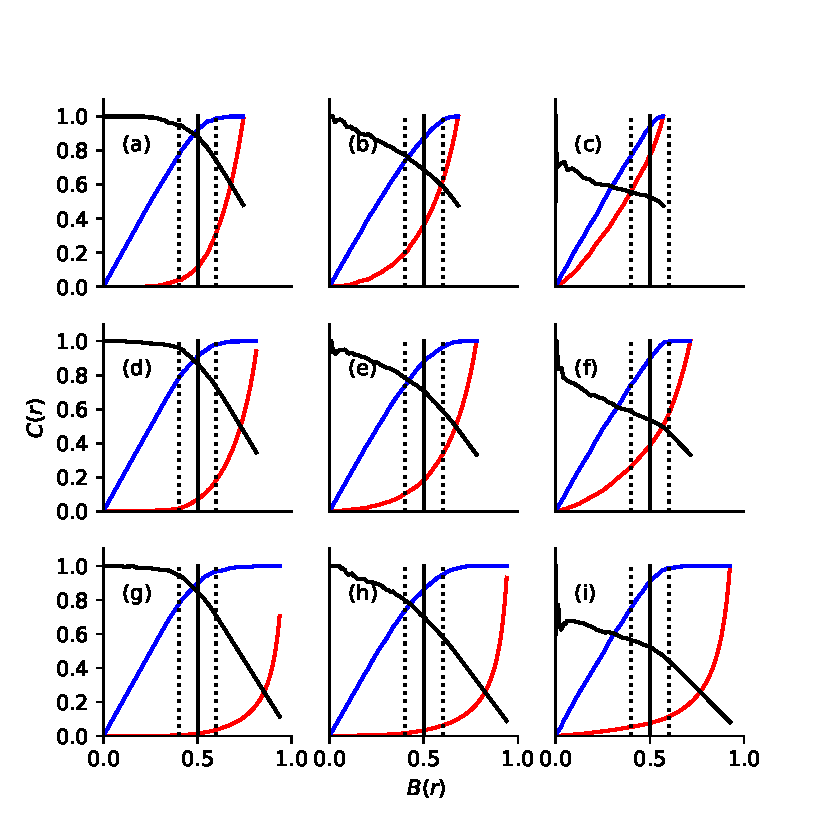
\includegraphics[scale=1]{Figures/Balance.pdf}
\caption{Plot of $B(r)$ against the precision $C(r)$ (black line), true positive rate $v(r)$ (blue) and false positive rate $u(r)$ (red) for our 9 example data sets. These curves are parameterised by $r$. }
\label{fig:balance}
\end{figure}


Figure \ref{fig:balance} shows $C(r)$ (black line) plotted against $r$ for our nine test data sets. Again, the way we built $B(r)$ allows us to explain in words what we are doing here. We can, for example, write about figure \ref{fig:balance}(e) that, "accepting a 60/40 imbalance in favour of positives our algorithm's predictions in favour of the positive class gave us a precision of $C(r_{60})=0.60$, compared to $C(r_b)=0.71$ at 50/50 balanced predictions." 

% The value in the top-right part of the figure is $C(r_b)$, the probability that a positive labelling is correct at balance. These values are strikingly similar for the data sets which have similar distributions for their `difficult' negative cases. Specifically: figures \ref{fig:balance} 
%As we have already seen, for $A$, a value near to $1/2$ implies the algorithm is no better than random and, as such, should not be used. A value near to $1$ indicates that the method is very accurate. Similarly, for $C(r_b)$, a value of 1 is an indication of accuracy, while the lowest possible accuracy is $P/(P+N)$, no more accurate than choosing a random individual. Note that, in figure \ref{fig:balance} (i), for example,  $P/(P+N)=1000/(1000+11000)=1/12$. So we could 'argue' that the algorithm is 6 times as accurate as random, since $C(r_b) \approx 6 P/(P+N)$. 

%The other way to address imbalances between true and false positive rates is to first assign a relative cost
% associated with each of them. So, for example, imagine a false negative is 10 times worse than a false positive, then a natural cost function 
%\begin{equation}
%10 (1-u(r)) + v(r)
%\end{equation}
%This is similar to the idea of bookmaker informedness \cite{powers2003precision}. It is the cost of making a mistake. For the data in \ref{fig:balance}(e) this cost is minimised when $r_{\mbox{min}}= -2.60$. This gives a balance of $B(r_{\mbox{min}})=0.646$ and a precision of $C(r_{\mbox{min}})=0.545$ (compared to $C(r_b)=0.734$ at balance).  We could write, that "by tuning our algorithm to favour true positives we reduce the precision fro $73.4$\% at balance, to $54.5$\%". In this particular example, the precision is now at a level comparable to that in figures \ref{fig:balance} (c), (f) and (i). We might think twice before putting such an algorithm in to production.


\subsection*{Relationship to F1 score}

\label{sec:others}

In this section we derive exact relationships between $B(r)$, precision, recall and the F1-score. In the Appendix, we show that $B(r)$ can be written in terms of the true positive rate, $v(r)$, the false positive rate, $u(r)$, and the density of scores of the negative class, $f_N(t)$, as
\begin{equation}
B(r) = \frac{P v(r)^2/2 + N \int_{t=r}^\infty f_N(t) v(t) dt }{P v(r) + N u(r)} .
 \label{eqn:Bdef}
\end{equation}
To make the relationships clear, we first break equation \ref{eqn:Bdef} in to two components,
\begin{equation}
B(r) = B_+(r) + B_-(r)  \label{eqn:Bpmdef} 
\end{equation}
such that
\begin{equation}
B_+(r) =  \frac{P v(r)^2/2}{P v(r) + N u(r)} = \frac{1}{2} v(r) C(r)   \label{eq:poscomponentB}
\end{equation}
and 
\begin{equation}
B_-(r) = \frac{N \int_{t=r}^\infty f_N(t) v(t) dt }{P v(r) + N u(r)}
 \label{eq:negcomponentB}
\end{equation}
These terms are plotted in figure \ref{fig:Bplot2}. We now look at these two terms individually.

\begin{figure}[tp]
\centering
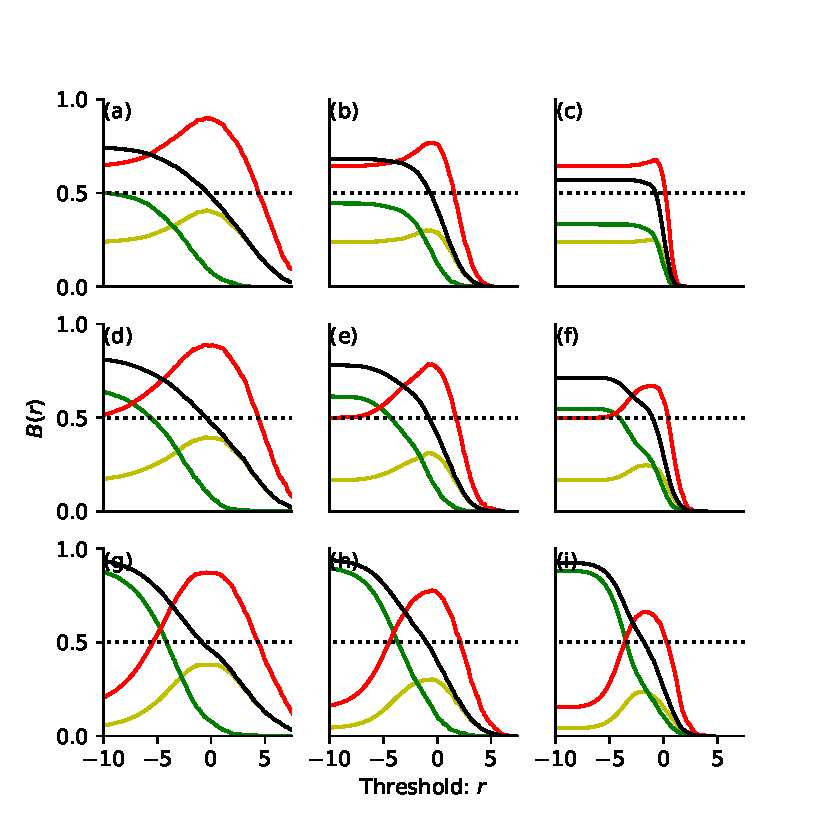
\includegraphics[scale=1]{Figures/Bplot2.pdf}
\caption{Plot of $B(r)$ for our 9 example data sets. The black line is $B(r)$. The dotted line at $1/2$ indicates the value at which the model is balanced. The yellow line is the component $B_+(r)$ (equation \ref{eq:poscomponentB}) and the green line is $B_-(r)$ (equation \ref{eq:negcomponentB}).  The red line is the $F_1(r)$ score (equation \ref{eq:F1}).}
\label{fig:Bplot2}
\end{figure}

Equation $B_+(r)$ is the precision multiplied by the true positive rate (recall), divided by two.

\paragraph{An AUC for the labelled members.} To interpret $B_-(r)$, define
\begin{equation}
\alpha(r) = P(S_P > S_N \mid S_P > r, S_N > r) = \frac{\int_{t=r}^\infty f_N(t) v(t) dt}{u(r) v(r)}  \label{eq:alpha}
\end{equation}
which is the probability that a randomly chosen true positive scores higher than a randomly chosen false positive, when the threshold is $r$. The numerator is $P(S_P > S_N, S_N > r)$, since $S_P>S_N>r$ implies that $S_P>r$, and the denominator is $P(S_P>r)P(S_N>r)$. In other words, $\alpha(r)$ is the area under the curve computed using only those members labelled positive, with $\alpha(-\infty)=A$. Since $1-C(r) = N u(r)/(P v(r) + N u(r))$, equation \ref{eq:negcomponentB} becomes $B_-(r) = v(r)\, \alpha(r) \left(1 - C(r)\right)$, and thus
\begin{equation}
B(r) = v(r) \left( \frac{C(r)}{2} + \alpha(r) \left(1 - C(r)\right) \right).  \label{eq:Bexact}
\end{equation}
This equation has a simple interpretation. $B(r)$ is the average, over all members labelled positive, of the proportion of the positive class which scores higher than that member. For a true positive this proportion is, on average, $v(r)/2$; for a false positive it is, on average, $\alpha(r) v(r)$. These two averages are weighted by the proportion of labelled members that are, respectively, true positives, $C(r)$, and false positives, $1-C(r)$.

\paragraph{Errors at the indistinguishability threshold.} It is useful to write equation \ref{eq:Bexact} in terms of the expected number of true positives, $TP = P v(r)$, false positives, $FP = N u(r)$, and false negatives, $FN = P (1 - v(r))$. Then $v(r) = TP/(TP+FN)$ and $C(r) = TP/(TP+FP)$, and setting $B(r_b)=1/2$ in equation \ref{eq:Bexact} gives
\[
\frac{TP}{TP+FN} \cdot \frac{TP/2 + \alpha FP}{TP+FP} = \frac{1}{2}
\]
where $\alpha = \alpha(r_b)$. Multiplying out gives $TP^2 + 2 \alpha \, TP \cdot FP = (TP+FN)(TP+FP)$, which simplifies to $(2\alpha - 1)\, TP \cdot FP = FN \, (TP+FP)$, or
\begin{equation}
\frac{FN}{FP} = \left( 2 \alpha(r_b) - 1 \right) C(r_b) . \label{eq:FNFP}
\end{equation}
Equation \ref{eq:FNFP} has three consequences. First, since $FN \geq 0$, we must have $\alpha(r_b) \geq 1/2$: at the indistinguishability threshold, true positives outrank false positives at least as often as would be expected by chance. Second, since $\alpha(r_b) \leq 1$ and $C(r_b)<1$ whenever there are false positives, $FN < FP$. Thus $TP + FP > TP + FN = P$, i.e. more members are labelled positive than there are members of the positive class, and recall is larger than precision, $v(r_b) > C(r_b)$. In other words, $r_b$ always lies below the precision-recall break-even point, which is the threshold at which $FP=FN$ and precision equals recall. Third, recall and the F1-score at $r_b$ are determined by the precision and $\alpha(r_b)$ alone. Since $FN/TP = (FN/FP)(FP/TP) = (2\alpha - 1) C \cdot (1-C)/C = (2\alpha - 1)(1-C)$, we have
\begin{equation}
v(r_b) = \frac{1}{1 + (2\alpha-1)(1-C)} \mbox{ and } F_1(r_b) = \frac{2C}{1 + C + (2\alpha-1) C (1-C)}  \label{eq:F1atrb}
\end{equation}
where $C=C(r_b)$, $\alpha=\alpha(r_b)$ and the F1-score is defined as,
\begin{equation}
F_1(r) =  \frac{2 C(r) v(r)}{C(r) + v(r)} = \frac{2 TP}{2 TP + FP + FN} .  \label{eq:F1}
\end{equation}

\paragraph{The threshold which maximises F1.} Figure \ref{fig:Bplot2} shows that the F1-score reaches a maximum at roughly the same point that $B(r)=1/2$. To see whether this is exact, we write $F_1(r) = 2 P v(r) / (P v(r) + N u(r) + P)$ and differentiate with respect to $r$. Using $v'(r) = -f_P(r)$ and $u'(r) = -f_N(r)$, the derivative is zero when $f_P(r) (N u(r) + P) = N v(r) f_N(r)$. Rearranging, this condition is
\begin{equation}
\eta(r) = \frac{F_1(r)}{2}, \mbox{ where } \eta(r) = \frac{P f_P(r)}{P f_P(r) + N f_N(r)}  \label{eq:F1max}
\end{equation}
is the probability that a member with score exactly $r$ is in the positive class. This is a known result: the F1-score is maximised at the threshold at which the probability of being positive equals half of the maximal F1-score \cite{lipton2014optimal}. Equation \ref{eq:F1max} depends only on the densities of scores at the threshold itself. In contrast, the condition $B(r_b) = 1/2$ depends, through $\alpha(r)$, on the distribution of all scores above the threshold. The two thresholds are therefore not the same in general. In the examples in figure \ref{fig:Bplot2} they are close, but this is a property of these particular data sets rather than a general identity.

A similar argument explains why the maxima of $F_1(r)$ and $B_+(r)$ are close. Let $s(r) = N f_N(r) / (P f_P(r))$ be the rate at which false positives are added, relative to true positives, as the threshold is lowered. At an interior maximum of $B_+(r) = TP^2/(2P(TP+FP))$ we must have $s(r) = 1 + 2FP/TP$, while at an interior maximum of $F_1(r) = 2TP/(TP+FP+P)$ we must have $s(r) = 1 + (FP+FN)/TP$. The two maxima thus coincide only if $FP = FN$ at that threshold, i.e. if the maximum lies exactly at the precision-recall break-even point.

The benchmark results in table \ref{tab:benchmarks} confirm the properties derived in this section. In all four cases more members are labelled positive at $r_b$ than there are members of the positive class, so that recall is larger than precision and $C(r_b)$ is below the precision at the break-even point. For logistic regression on the Mammography data, twice as many regions are labelled positive as there are positives. The ratio $FN/FP$ agreed with $(2\alpha(r_b)-1)C(r_b)$ (equation \ref{eq:FNFP}) to within $0.006$ in all four cases. On the Adult data, the F1-score at $r_b$ is within 0.005 of its maximum, but on the Mammography data it is 0.11--0.13 lower, illustrating that the indistinguishability threshold and the F1-optimal threshold need not coincide.

\section*{Discussion}

Every quantity in this article answers a question that can be stated in words, in terms of images that contain cats and images that do not, and every answer is a proportion that can be reported as a percentage. Table \ref{tab:words} lists these questions. Some of them, such as the AUC, were already known; the others follow from the same idea of comparing randomly chosen pairs of members. Even the exact results in the section {\it Relationship to F1 score} can be stated in this way. For example, at the indistinguishability threshold the algorithm always labels more images as cats than there are cats, so that the proportion of cats it finds is always larger than the proportion of labelled images that are cats. The F1-score is the exception. It is the harmonic mean of precision and recall, and it does not answer any question that a user of the algorithm would naturally ask \cite{hand2018note, hand2021f}.

\begin{table}[tp]
\centering
\small
\begin{tabular}{p{2.3cm}p{9.4cm}}
\toprule
Measure & Question it answers \\
\midrule
$A$ (AUC) & If the algorithm is shown one image that contains a cat and one that does not, how often does it give the higher score to the image containing the cat? \\[3pt]
$B(r)$ & If we pick one image labelled as a cat and one image that really contains a cat, how often does the real cat have the higher score? \\[3pt]
$r_b$ & At what threshold is an image labelled as a cat equally likely as an image of a real cat to have the higher score? \\[3pt]
$C(r_b)$ & When the algorithm is tuned so that it can no longer distinguish the images it labels as cats from images that really contain cats, how often does an image labelled as a cat actually contain one? \\[3pt]
$v(r_b)$ & At that threshold, what proportion of the images containing cats are labelled as cats? \\[3pt]
$\alpha(r_b)$ & Among the images labelled as cats, how often does an image containing a cat have a higher score than an image that does not? \\[3pt]
$C(r_{60})$ & If we accept that a real cat scores higher than an image labelled as a cat 60\% of the time, how often does an image labelled as a cat actually contain one? \\
\bottomrule
\end{tabular}
\caption{The measures used in this article and the questions they answer. Each answer is a proportion that can be reported as a percentage.}
\label{tab:words}
\end{table}

Being able to state a measure in words matters because the people who decide whether, and how, to use a machine learning algorithm are rarely machine learning specialists. A clinician deciding whether to introduce a screening tool, a manager deciding whether to automate a task or a regulator assessing a claim about an algorithm needs to know what the reported numbers mean for the cases they will actually see. In the Mammography example in the section {\it Two benchmark data sets}, we can tell a radiologist that, when the gradient boosting classifier is tuned to the indistinguishability threshold, about half of the regions it flags contain microcalcifications, so that each correct detection comes with roughly one false alarm, and that it finds 72\% of the regions that do contain microcalcifications, so that 28\% are missed. These statements translate directly into the workload that the tool creates and the cases that it misses, and the radiologist can judge for themselves whether this is acceptable. The same data set illustrates the danger of reporting a measure without saying what it means. Both classifiers have an AUC of 0.92, which sounds excellent, but the AUC answers a question that a radiologist never faces, about pairs of regions of which exactly one is known to contain microcalcifications, and it hides a large difference in how often the flagged regions are correct.

Measures stated in words also make it possible to discuss trade-offs. No single measure can capture the performance of an algorithm, because there is always a trade-off between the two types of error, false positives and false negatives \cite{neyman1933ix, scott2007performance}. In medicine in particular, the costs and benefits of the two types of error should be weighed and the algorithm assessed in light of them \cite{obuchowski2018receiver, chu1999introduction, care2018new}. When these costs are known, the threshold can be chosen to minimise the expected cost \cite{elkan2001foundations}. But costs are often difficult to specify in advance, and they are rarely specified when an algorithm is first developed. Statements in words give users a way of finding the trade-off that suits them. For example, we can say that accepting that a real cat scores higher than an image labelled as a cat 60\% of the time, rather than 50\%, increases the proportion of cats that are found, but reduces the proportion of labelled images that are cats from 71\% to 60\% (figure \ref{fig:balance}e). Both sides of the trade-off are expressed in the same terms as the measure itself.

The indistinguishability threshold has two further practical advantages. First, it depends only on the ranking of the scores and not on their values. Unlike the threshold $r=0$ for logistic regression, or the threshold which maximises the F1-score (equation \ref{eq:F1max}), it does not require the scores to be calibrated probabilities. Second, it is not affected by adding members that are easy to classify, since these are never labelled positive. In our artificial data sets, adding easy cases increased the AUC but left $C(r_b)$ almost unchanged, and in the benchmark data, removing the easiest half of the negative members reduced the AUC but left $C(r_b)$ exactly unchanged.

The measure also has limitations. Like any precision, $C(r_b)$ depends on the relative number of positive members and negative members that are difficult to classify, so it should be compared across data sets with care. This dependence is, however, also what makes it useful in an application: it tells users what proportion of flagged cases will be correct in the population to which the algorithm is applied. Furthermore, the labelled and positive sets are indistinguishable only in the sense of stochastic equality, not in the sense of having identical distributions of scores. Finally, the idea of an indistinguishability threshold may be useful beyond evaluation. In boosting \cite{schapire2003boosting}, for example, a model could first be fitted to all members, and a new model then fitted to the members with scores greater than $r_b$, potentially improving the fit in an iterative way.

The development of many machine learning algorithms takes place before the trade-off between error types in a particular application has been specified. In such situations, precision at the indistinguishability threshold combines the respective advantages of AUC, that it can be explained simply in words, and of the F1-score, that it is not inflated by adding cases that are easy to classify. We would therefore encourage researchers to report $C(r_b)$, together with the recall at the same threshold, $v(r_b)$, and to state both in words: {\it when the algorithm is tuned so that it can no longer distinguish the cases it flags from real cases, X\% of the flagged cases are real, and Y\% of the real cases are flagged.} Reported in this way, the performance of an algorithm can be understood, questioned and discussed by the people who will use it.

\section*{Acknowledgements}

Thanks to Daniel Gedon and Andre Teixeira for feedback. 

\section*{Appendix: Properties and implementation of $B(r)$}
\label{app:B}

In this appendix we show how $B(r)$ can be calculated. As with $A$ the pairwise nature of the test means it is straightforward to implement a randomised version of $B(r)$. For each value of $r$ we sample, with or without replacement, $n$ members of the positive class. Then we sample $n$ members from the set labelled positive when the threshold is greater than $r$. Pairwise comparison of the scores of these two sets gives $B(r)$ . This method becomes less reliable for large values of $r$, since the size of the positive labelled class becomes small and all the comparisons will be made to a small number of positively labelled images. 

Another way to calculate $B(r)$, following the AUC approach to estimating $A$, is by integration over the true positive rate, $v(r)$, and the false positive rate, $u(r)$. We now derive the appropriate integral. First, let $S_R$ be the score of a randomly chosen member of the data set and $S_P$ the score of a randomly chosen member of the positive class. The probability that $S_R$ is less than $S_P$, given that $S_R$ is greater than $r$, is then written as $P(S_R<S_P | S_R>r)$. It is this probability we call $B(r)$.

Our approach to finding an expression for $B(r)$ is to look separately at the case where $S_R$ is from a negative member and a positive member. We can use the law of total probability to give 
\begin{eqnarray}
B(r) &= &P(S_R < S_P | S_R>r) \nonumber \\
& = & P(S_R < S_P | S_{R} > r , R = + ) \cdot P( R = + | S_R > r )  \nonumber \\
&&  + P(S_R < S_P | S_R>r, R= - ) \cdot P( R = - | S_R>r ) \label{eqn:totprobstep} 
\end{eqnarray}
where $+$ and $-$ are respectively the events that the chosen individuals are in the positive and negative classes. If an individual is chosen at random then 
\begin{equation}
P( R = + | S_R>r ) =   \frac{P v(r)}{P v(r) + N u(r)}  \mbox{ and }  P( R = - | S_R>r ) =   \frac{N u(r)}{P v(r) + N u(r)} \label{eqn:probbe}
\end{equation}
Furthermore,
\begin{eqnarray}
P(S_R < S_P | S_{R} > r ,  R = +   ) & = & \frac{P(S_R < S_P \cap S_{R} > r ,  R = +  )}{P(S_{R} > r ,  R = +  )} \nonumber \\
& = & \frac{\int_{t=r}^\infty \int_{s=t}^\infty f_P(t) f_P(s) ds dt}{\int_{t=r}^\infty f_P(t) dt} \nonumber \\
& = & \frac{\int_{t=r}^\infty f_P(t) v(t) dt}{v(r)} \label{eqn:posstep}
\end{eqnarray}
Since the derivative of $v(r)$ is equal to $-f_P(r)$ we can change variable to $v$ in the integral in the numerator to get
 \begin{eqnarray}
\int_{t=r}^\infty f_P(t) v(t) dt =  \int_{t=r}^\infty v(t) \left( -v'(t) \right) dt = \int_{0}^{v(r)} v \, dv = \frac{v(r)^2}{2}
\end{eqnarray}
and thus simplify to get
\begin{equation}
P(S_R < S_P | S_{R} > r ,  R = +   ) = \frac{v(r)}{2} \label{eqn:posstepfinal}
\end{equation}
We can follow similar steps for the case that $R$ is negative to get,
\begin{equation}
P(S_R < S_P | S_{R} > r ,  R = -   ) = \frac{\int_{t=r}^\infty f_N(t) v(t) dt}{u(r)}  \label{eqn:negstep}
\end{equation}
Substituting \ref{eqn:probbe}, \ref{eqn:posstepfinal} and \ref{eqn:negstep} in to equation \ref{eqn:totprobstep} gives equation \ref{eqn:Bdef} in the section {\it Relationship to F1 score}. This equation is plotted as the black line in figure \ref{fig:Bplot}. As $r \rightarrow -\infty$, $v(r)$ and $u(r)$ tend to one and $\int_{t=r}^\infty f_N(t) v(t) dt$ tends to $A$ (equation \ref{eq:SPgreaterSN2}), so that
\[
B(-\infty) = \frac{P/2 + N A}{N + P} 
\]
while $B(r) \leq v(r) \rightarrow 0$ as $r \rightarrow \infty$. 

In between, $B(r)$ always decreases as $r$ increases. To see this, write $D(r) = P v(r) + N u(r)$ for the denominator of equation \ref{eqn:Bdef}. The derivative of the numerator is $P v(r) v'(r) - N f_N(r) v(r) = v(r) D'(r)$, so that
\[
B'(r) = \frac{D'(r)}{D(r)} \left( v(r) - B(r) \right).
\]
Since $D'(r) = -(P f_P(r) + N f_N(r)) \leq 0$ and, from equation \ref{eq:Bexact}, $B(r) \leq v(r) \left(1 - C(r)/2\right) < v(r)$, we have $B'(r) \leq 0$. Thus $B(r)$ decreases from $B(-\infty)$ to zero, and a threshold $r_b$ with $B(r_b)=1/2$ exists if and only if $B(-\infty) \geq 1/2$, which is equivalent to $A \geq 1/2$. In other words, the indistinguishability threshold exists whenever the algorithm does at least as well as random guessing, and it is unique wherever the densities of scores are positive. It is identified as the point in figure \ref{fig:Bplot} where $B(r)$ crosses the dotted line at $1/2$, and is plotted as the vertical dotted line in figure \ref{fig:Distribution}.

\bibliographystyle{ieeetr}
%\bibliographystyle{plain}

\bibliography{ref}

\end{document}

\end{document}

